\documentclass[sigconf, nonacm]{acmart}

%%% do not modify the following VLDB block %%
%%% VLDB block start %%%
\usepackage{pvldb}
%%% VLDB block end %%%

\usepackage{booktabs}
\usepackage{tikz}
\usetikzlibrary{arrows.meta, positioning}
\definecolor{pcablue}{HTML}{4C72B0}
\definecolor{ballorange}{HTML}{DD8452}

\renewcommand\vldbdoi{XX.XX/XXX.XX}
\renewcommand\vldbpages{XXX-XXX}
\renewcommand\vldbavailabilityurl{https://github.com/taiwuchiang-gmail/hierarchical-pca-search}

\begin{document}

\title{Exact Nearest-Neighbor Search with Composable Lower Bounds:
Self-Configuring Hierarchical Pruning, In RAM and Out of Core}

\author{Tai-Wu Chiang}
\orcid{0009-0004-7062-9346}
\email{twchiang@utexas.edu}
\affiliation{%
  \institution{Independent Researcher}
  \city{California}
  \country{USA}}

\begin{abstract}
Applications that cannot tolerate a missed true neighbor---deduplication,
medical and legal retrieval, scientific analysis---need \emph{exact}
nearest-neighbor search, for which the standard tool is a cheap lower bound
that prunes candidates without computing full distances. We develop such
bounds from truncated PCA projections, which are tight precisely when
variance concentrates in few dimensions, and observe that they are one
member of a \emph{family}: any region that provably contains a set of
points yields an exact lower bound via the query-to-region distance, and
different region shapes are tight for different data structures. We compose
two complementary families---PCA truncation (tight for linearly correlated
data) and
triangle-inequality ball bounds around $k$-means centroids (tight for
clustered data, and exact for \emph{any} centers, so approximation quality
affects only speed, never correctness)---into a single exact cascade. Because
neither family helps on all data, the index \emph{configures itself} from a
sample: cascade widths are chosen from the eigenvalue curve (fixed widths
tuned for 128-dimensional descriptors misread 1536-dimensional OpenAI
embeddings as unprunable; widths placed at fixed variance targets recover
them), and a three-tier diagnostic---eigen curve, beyond-covariance
statistics, then a measured trial of the real cascade---decides which levels
to build. We report results in hardware-independent work units alongside
wall-clock, because wall-clock proved regime-dependent (the same algorithm
measured $4.7\times$, $3.6\times$, $2.7\times$, and parity under changes of
numeric type, machine load, and implementation tuning) while its work counts
never moved. On four real datasets spanning 96--1536 dimensions (SIFT1M,
GIST1M, DBpedia-OpenAI-1M, DEEP10M), exact 1-NN costs $3.9$--$20.8\times$
less work than a scan, with wall-clock gains \emph{growing} with
dimensionality ($2.6\times$ at 128-D to $6.2\times$ at 960-D): brute force
pays the full dimension per point while the cascade pays for intrinsic
structure. Exact $k$-NN generalizes the pruning radius to the $k$-th order
statistic over evaluated points; it wins to $k\approx10$ and honestly loses
in RAM at $k=100$. Out of core, the cascade's fetch set concentrates in few
$k$-means clusters (27 of 1024 on the embeddings), and a measured two-tier
layout under \texttt{O\_DIRECT} cold reads answers exact queries
$7$--$17\times$ faster than a full disk scan while reading
$40$--$730\times$ fewer bytes. Against ADSampling, the state-of-the-art
statistical distance-comparison pruner, our in-RAM work counts are mixed
(we win at 96--128 dimensions, it wins on the embeddings), but its
$\Delta d = 32$-dimension floor forces it to touch \emph{every} vector, so
it cannot leave RAM: deterministic bounds pay precisely where bytes are
expensive. Exactness is verified on every query of every experiment. All
code, diagnostics, and experiments are public.
\end{abstract}

\maketitle
\vldbtopmatter

\section{Introduction}

Finding the exact nearest neighbor in a large, high-dimensional dataset is
bottlenecked by the cost of computing full distances. Approximate methods
(LSH~\cite{lsh}, HNSW~\cite{hnsw}, IVF~\cite{faiss}) trade recall for
speed; for applications where a missed true neighbor is
unacceptable---deduplication, medical and legal retrieval, scientific
analysis---the alternative is exact pruning in the GEMINI
tradition~\cite{gemini}: compute a cheap \emph{lower bound} on each
candidate's distance, and discard the candidate if the bound already
exceeds the best distance found so far. Our starting point is such a bound
from truncated PCA projections (\S\ref{sec:pca}): after rotating the data
onto its principal axes, the distance between $k$-dimensional prefixes
lower-bounds the true distance, so a cascade of progressively finer
prefixes---seeded by a dynamic Top-$K$ probe---prunes over 99.9\% of the
SIFT1M dataset while returning provably exact results.\footnote{Preliminary
versions of this work appeared as two self-archived reports
(doi:10.5281/zenodo.21387358, doi:10.5281/zenodo.22199955). This paper
merges, extends, and supersedes them: the $k$-NN generalization, the
eigen-curve width selection, three of the four datasets, the measured
out-of-core results, and the ADSampling baseline are new.}

That bound has a blind spot, and it is structural. PCA truncation is tight
exactly when variance concentrates in few principal directions---linearly
correlated data. Datasets whose structure is \emph{clustered} rather than
correlated can present a flat eigenvalue spectrum, collapsing the PCA
cascade toward brute force, while remaining highly compressible in a
different sense: points huddle near a modest number of centroids. No single
bound family serves all data, and, worse, a practitioner has no way to know
before building an index which family---if any---their data supports.

This paper makes two moves. First, \textbf{exact bounds compose}: the
maximum of valid lower bounds is a valid lower bound, so bound families with
complementary blind spots can share one cascade. We add a
triangle-inequality \emph{ball bound} around $k$-means centroids---the
clustered-data complement of PCA truncation---and show that it is exact for
\emph{any} choice of centers: clustering quality affects only pruning power,
never correctness. Second, \textbf{the composition is chosen by
measurement}: a three-tier diagnostic, run on a sample in seconds, rates the
PCA levels from the eigenvalue decay, detects structure beyond the
covariance with two cheap statistics, and---because we show statistics alone
mispredict in both directions---settles the question with a measured trial
of the real cascade, emitting an \textsc{add}/\textsc{skip} verdict per
level.

There is also an economic motivation. An exhaustive flat scan requires the
entire dataset resident in RAM---the most expensive byte in the machine,
running roughly an order of magnitude above NVMe per byte, and more under
supply pressure. The pruning cascade needs only its metadata resident: 8--40
bytes per vector versus 512 bytes per vector for \texttt{fp32} data. At one
billion vectors this is 8--40\,GB of RAM versus 512\,GB---a commodity box
versus a specialty one---with exactness preserved.

Our contributions:
\begin{enumerate}
\item \textbf{Exact hierarchical pruning from composable bounds}: a
  PCA-prefix cascade with a dynamic Top-$K$ pruning radius, unified with
  the triangle-inequality ball bound under a containing-region principle
  in which each bound family covers the other's structural blind spot
  (\S\ref{sec:theory}).
\item A \textbf{composed exact cascade}---ball level plus PCA levels---with
  a radius re-probe, generalized to exact \textbf{$k$-NN} via the $k$-th
  order statistic over evaluated points. Storage overhead is $\sim$8 bytes
  per point (\S\ref{sec:algorithm}).
\item \textbf{Self-configuration that includes the cascade widths}: levels
  are placed at fixed cumulative-variance targets on the eigenvalue curve
  (a fixed ladder is silently calibrated to one dimensionality and misreads
  others), then the three-tier funnel---statistics nominate, measurement
  decides---rules on each level, with verdicts derived from measured work
  ratios; negative verdicts included (\S\ref{sec:funnel}).
\item \textbf{Full-scale evidence on four real datasets} (96--1536
  dimensions, $10^6$--$10^7$ points) in hardware-independent work units,
  with wall-clock as cost-model validation, negative controls, and
  sample-to-full-scale extrapolation checks (\S\ref{sec:eval}).
\item A \textbf{measured out-of-core design}: the fetch set's cluster
  locality, a two-tier on-disk layout, and cold-read benchmarks under
  \texttt{O\_DIRECT} showing exact search $7$--$17\times$ faster than a
  full disk scan (\S\ref{sec:ooc}).
\item An \textbf{ADSampling baseline} in a shared work currency, locating
  the honest boundary between statistical and deterministic pruning
  (\S\ref{sec:ads}).
\end{enumerate}

\section{Background and Related Work}

\textbf{Lineage.} Neither bound family is new, and we do not claim
otherwise. Lower-bounding by dimensionality reduction descends from the
GEMINI framework~\cite{gemini} and the VA-file~\cite{vafile}. Pruning by
the triangle inequality around reference points is the basis of ball
trees~\cite{balltree}, vantage-point trees~\cite{vptree}, GNAT~\cite{gnat},
and Elkan's accelerated $k$-means~\cite{elkan}. The approximate cousins are
FAISS IVF~\cite{faiss} (the same $k$-means geometry without exactness) and
OPQ~\cite{opq} (a per-cell rotation, the ellipsoid rung of the shape ladder
in \S\ref{sec:theory}). Disk-resident ANN systems such as
DiskANN~\cite{diskann} and SPANN~\cite{spann} target the same
memory-economics regime we do, but are approximate. Closest in mechanism is
ADSampling~\cite{adsampling}, which also evaluates incremental prefix
distances after a rotation, but replaces the deterministic bound with a
sequential hypothesis test under a \emph{random} rotation (its layout-level
successor is PDX~\cite{pdx}); we measure against it directly in
\S\ref{sec:ads}. Our contribution is the \emph{exact composition} of the
two bound families in one cascade, the \emph{measured self-configuration}
(including the cascade widths themselves), and a diagnostic that also tells
the practitioner when to walk away.

\section{Composable Exact Bounds}
\label{sec:theory}

\subsection{The PCA Truncation Bound}
\label{sec:pca}

Let $X, Y \in \mathbb{R}^d$ and let $X', Y'$ be their images under the
orthogonal rotation onto the dataset's principal axes. Rotation preserves
the squared Euclidean distance,
$L_2^2(X, Y) = L_2^2(X', Y') = \sum_{i=1}^{d} (x'_i - y'_i)^2$.
Let $T_k$ retain the first $k$ coordinates.

\begin{lemma}
\label{lem:pca}
For any truncation width $k < d$,
$L_2^2\!\bigl(T_k(X'), T_k(Y')\bigr) \le L_2^2(X, Y)$.
\end{lemma}

\begin{proof}
The true squared distance is a sum of $d$ non-negative terms; the truncated
distance is the sum of the first $k$ of the same terms, and
$\sum_{i=k+1}^{d} (x'_i - y'_i)^2 \ge 0$.
\end{proof}

If the prefix distance to a candidate already exceeds the current search
radius $r$, the candidate is discarded without ever computing its full
distance---the GEMINI no-false-dismissal condition~\cite{gemini}. Two
choices make the bound an algorithm. First, \emph{which rotation}: any
orthogonal rotation satisfies Lemma~\ref{lem:pca}; PCA makes the bound
\emph{tight}, since by the Karhunen--Lo\`eve theorem it packs the maximum
variance---and hence, on average, the largest share of any pairwise
distance---into the first $k$ coordinates
(quantified in Eq.~(\ref{eq:tightness})). Exactness is unconditional;
quality is not, a separation that recurs throughout this paper. Second,
\emph{where the radius comes from}: rather than a static threshold, a
Top-$K$ probe at the coarsest width computes exact distances for the $K$
most promising candidates ($K = 50$) and sets $r$ to their minimum. Because
the prefix distance is a lower bound, this radius is mathematically safe
from the first comparison on, with no prior knowledge of the neighbor
distance. A cascade of progressively finer prefixes then re-prunes the
survivors at each width; on SIFT1M, widths $(8,16,32,64)$ discard all but
an average of 564 of $10^6$ vectors before any full-dimensional
evaluation, and \S\ref{sec:funnel} replaces the fixed widths with ones
derived from the data's own eigenvalue curve.

\subsection{The Containing-Region Principle}

Let $R \subseteq \mathbb{R}^d$ be any region that provably contains a set of
points $C$. Then for every $p \in C$ and any query $q$,
\begin{equation}
\lVert q - p \rVert \;\ge\; \mathrm{dist}(q, R),
\end{equation}
so $\mathrm{dist}(q,R)$ is an exact pruning bound for every member of $C$
at once. A bound family is therefore a \emph{shape} family, and a shape is
admissible when (a) containment is guaranteed and (b) $\mathrm{dist}(q,R)$
is cheap. Table~\ref{tab:shapes} lists the natural ladder. Each geometric
family is the twin of a quantizer family: a quantizer's
codeword-plus-distortion model \emph{is} a containing region. We use the
first two rungs; the others are available under the same principle.

\begin{table}[t]
\caption{Shape families and their exact bounds. Each is tight for a
different data structure; each mirrors a quantizer family.}
\label{tab:shapes}
\small
\begin{tabular}{@{}llll@{}}
\toprule
Shape & Bound cost & Tight for & Quantizer twin \\
\midrule
ball & $|\,\lVert q{-}c\rVert - d_p\,|$ & clusters & VQ \\
ellipsoid & per-axis scaled & stretched clusters & OPQ \\
slab & projection residual & local low rank & local PCA \\
cone$\times$annulus & closed form & radial/gain data & gain--shape \\
\bottomrule
\end{tabular}
\end{table}

\subsection{The Ball Bound}

Cluster the dataset with $k$-means. For each point $p$ assigned to centroid
$c$, store the scalar $d_p = \lVert p - c \rVert$ once, offline. At query
time, compute the $k$ centroid distances $\lVert q - c_j \rVert$ (with
$k \ll N$), and the triangle inequality gives, for every point,
\begin{equation}
\label{eq:ball}
\lVert q - p \rVert \;\ge\; \bigl|\, \lVert q - c_{a(p)} \rVert - d_p \,\bigr|,
\end{equation}
where $a(p)$ is $p$'s cluster. Evaluating (\ref{eq:ball}) for all $N$ points
requires one gather and one subtraction per point---\emph{no distance
computations}. A coarser, per-cluster form uses the cluster radius
$R_j = \max_{p \in j} d_p$: if $\lVert q - c_j \rVert - R_j$ exceeds the
current radius, the entire cluster is eliminated in one comparison, which in
an out-of-core layout skips a whole contiguous block (\S\ref{sec:layout}).

\subsection{Exactness Is Unconditional; Quality Is Not}

Inequality~(\ref{eq:ball}) is the triangle inequality: it holds for
\emph{any} reference points whatsoever. $k$-means enters only because it
minimizes the mean $d_p^2$, which is what makes the bound \emph{tight}. Three
corollaries follow. Stale centers remain correct as the dataset drifts
(pruning degrades gracefully; re-cluster when a diagnostic says so).
Insertion is $O(1)$: assign the new point to its nearest existing centroid
and store $d_p$; no re-clustering is required for correctness. And the
composed index inherits the PCA bound's property (\S\ref{sec:pca}) in
mirror image: there, any
orthogonal rotation is exact and PCA makes it tight; here, any centers are
exact and $k$-means makes them tight. Since the maximum of lower bounds is a
lower bound, the two families compose freely in one cascade.

\subsection{Complementarity}

\begin{figure}[t]
\centering
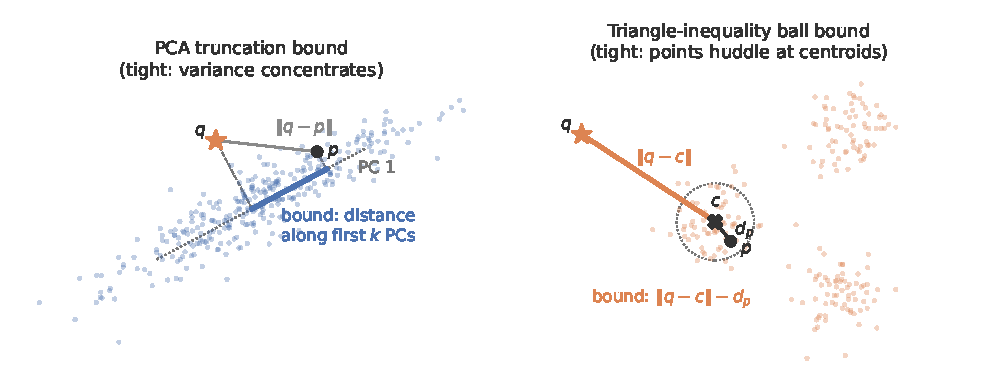
\includegraphics[width=\linewidth]{fig_bounds.pdf}
\caption{The two exact bound geometries. Left: the PCA truncation bound is
the distance between the projections onto the first $k$ principal
components---tight when variance concentrates along few directions. Right:
the ball bound $\lVert q-c \rVert - d_p$ from the triangle
inequality---tight when points huddle near their centroids. Each is loose
exactly where the other is tight.}
\label{fig:bounds}
\end{figure}

PCA truncation is tight iff the eigenvalue spectrum decays steeply---a
\emph{global, linear} property (Figure~\ref{fig:bounds}, left). The ball bound is tight iff points sit close
to centroids relative to the spread of $\lVert q - c \rVert$---a
\emph{local} property that holds for multimodal data and, more generally,
for data of low intrinsic dimension, where $d_p$ and the centroid distances
spread widely instead of concentrating. The blind spots are disjoint by
construction. Our clearest demonstration: a synthetic dataset of 512 tight
clusters whose centers span all dimensions has a nearly flat spectrum (95\%
of variance needs 111 of 128 dimensions; the PCA cascade manages
$2.1\times$), yet the ball bound prunes to 3\% before a single projection is
computed.

\section{The Self-Configuration Funnel}
\label{sec:funnel}

The funnel answers, from a sample and in seconds, ``which levels should this
index have for \emph{my} data?'' Figure~\ref{fig:funnel} shows its shape:
two statistical tiers that may only \emph{nominate}, and one measured tier
that alone \emph{decides}.

\begin{figure}[t]
\centering
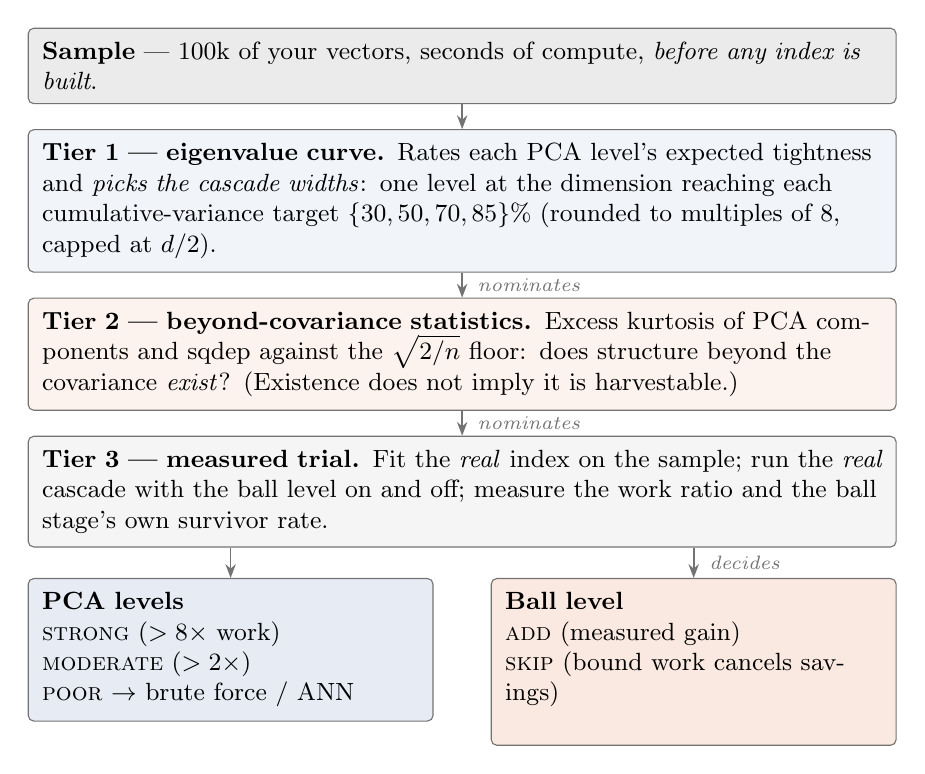
\begin{tikzpicture}[
  font=\small,
  box/.style={rectangle, rounded corners=2pt, draw=black!55, align=left,
              inner sep=5pt, text width=0.88\linewidth},
  vbox/.style={rectangle, rounded corners=2pt, draw=black!55, align=left,
              inner sep=5pt, text width=0.395\linewidth},
  arr/.style={-{Stealth[length=5pt]}, semithick, black!55},
  lbl/.style={font=\scriptsize\itshape, black!55, midway, right=2pt},
  node distance=9pt
]
\node (sample) [box, fill=black!8] {\textbf{Sample} --- 100k of your
  vectors, seconds of compute, \emph{before any index is built}.};
\node (t1) [box, fill=pcablue!8, below=of sample]
  {\textbf{Tier 1 --- eigenvalue curve.} Rates each PCA level's expected
  tightness and \emph{picks the cascade widths}: one level at the
  dimension reaching each cumulative-variance target
  $\{30,50,70,85\}\%$ (rounded to multiples of 8, capped at $d/2$).};
\node (t2) [box, fill=ballorange!10, below=of t1]
  {\textbf{Tier 2 --- beyond-covariance statistics.} Excess kurtosis of
  PCA components and $\mathrm{sqdep}$ against the $\sqrt{2/n}$ floor:
  does structure beyond the covariance \emph{exist}? (Existence does not
  imply it is harvestable.)};
\node (t3) [box, fill=black!4, below=of t2]
  {\textbf{Tier 3 --- measured trial.} Fit the \emph{real} index on the
  sample; run the \emph{real} cascade with the ball level on and off;
  measure the work ratio and the ball stage's own survivor rate.};
\node (vp) [vbox, fill=pcablue!14, below=11pt of t3.south west,
  anchor=north west]
  {\textbf{PCA levels}\\ \textsc{strong} ($>8\times$ work)\\
  \textsc{moderate} ($>2\times$)\\ \textsc{poor} $\to$ brute force / ANN};
\node (vb) [vbox, fill=ballorange!18, below=11pt of t3.south east,
  anchor=north east]
  {\textbf{Ball level}\\ \textsc{add} (measured gain)\\
  \textsc{skip} (bound work cancels savings)\\ \mbox{}};
\draw[arr] (sample) -- (t1);
\draw[arr] (t1) -- (t2) node[lbl] {nominates};
\draw[arr] (t2) -- (t3) node[lbl] {nominates};
\draw[arr] (t3.south -| vp.north) -- (vp.north);
\draw[arr] (t3.south -| vb.north) -- (vb.north)
  node[lbl, right=2pt] {decides};
\end{tikzpicture}
\caption{The self-configuration funnel. Tiers 1--2 are statistics: cheap,
and only allowed to \emph{nominate} (tier 1 also derives the cascade
widths from the eigenvalue curve). Tier 3 is a measured trial of the real
cascade and alone \emph{decides}. \S\ref{sec:extrap} shows the sample
verdicts holding at $10^6$--$10^7$ scale; the tier-2 mispredictions below
(SIFT and latent-8, in opposite directions) are why no statistic can
replace the trial.}
\label{fig:funnel}
\end{figure}

\textbf{Tier 1 --- eigenvalue decay, which also \emph{picks} the
widths.} Fit PCA on a sample. The eigenvalue curve is not merely a
heuristic signal: in the PCA basis the coordinates of the difference
between two independently drawn points are uncorrelated with variances
$2\lambda_i$, so for typical candidate pairs
\begin{equation}
\label{eq:tightness}
\frac{\mathbb{E}\,L_2^2\bigl(T_k(X'), T_k(Y')\bigr)}
     {\mathbb{E}\,L_2^2(X, Y)}
\;=\;
\frac{\sum_{i \le k} \lambda_i}{\sum_{i} \lambda_i},
\end{equation}
the cumulative explained variance at $k$. The curve therefore reads
directly as the \emph{expected fractional tightness} of the width-$k$
bound on the very population the cascade prunes---each dataset's curve is
its prunability signature (Figure~\ref{fig:eigen}). Two blind spots
follow from the same statement, and each motivates a later tier.
Equation~(\ref{eq:tightness}) is an expectation over pairs, while pruning
is a tail event---a candidate is discarded only when its prefix distance
clears the radius---so scalar summaries of the curve can mislead: GIST1M
needs 303 of 960 dimensions for 95\% variance, a ``flat spectrum'' by the
usual standard, yet its steep \emph{head} (48\% by eight components) is
what the early levels price, and the measured verdict is \textsc{strong}.
And the spectrum is second-order only: clustered structure that no
rotation can expose is invisible to it, which is what tier 2 screens for
and tier 3 settles.

\begin{figure}[t]
\centering
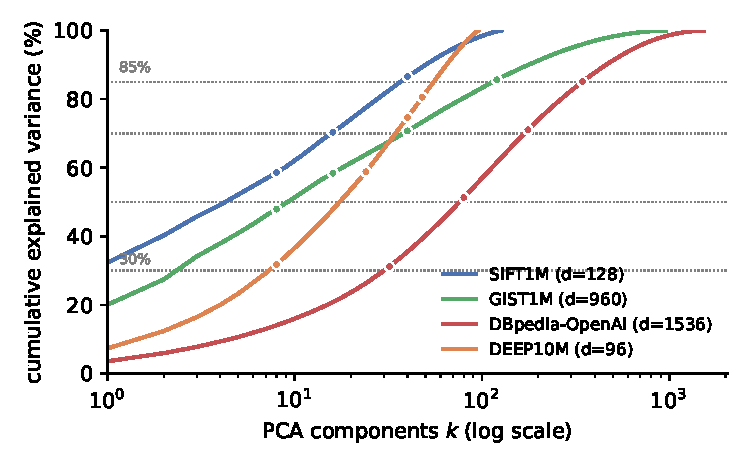
\includegraphics[width=\linewidth]{fig_eigen.pdf}
\caption{Cumulative explained variance on 100k samples (log-scale
components): each dataset's prunability signature, since by
Eq.~(\ref{eq:tightness}) the curve is the expected fractional tightness
of a width-$k$ bound. Dots mark the widths the funnel selects at the
$\{30,50,70,85\}\%$ targets (dotted lines). SIFT and GIST are
steep-headed; DBpedia's curve is shifted right---the reason a fixed
$d{=}128$ ladder misreads it as unprunable; DEEP is flattest, matching
its \textsc{moderate} verdict, and its last width sits below the 85\%
line because of the $d/2$ cap.}
\label{fig:eigen}
\end{figure}

Preliminary
versions of this work used a fixed ladder $(8,16,32,64)$---which, we
discovered, is silently calibrated to $d \approx 128$: on 1536-dimensional
OpenAI embeddings it stops at 4\% of the dimensions, prunes almost nothing
(68\% survivors after the 64-D stage), and the funnel misreads eminently
prunable data as hopeless. The fix makes tier 1 constructive: place one
level at the dimension reaching each cumulative-variance target
$\{30, 50, 70, 85\}\%$, rounded up to a multiple of 8 and capped at $d/2$.
Measured against hand-tuned ladders on 100k samples (work ratio), the rule
ties SIFT ($8.2\times$ vs $8.5\times$) and \emph{wins} GIST1M
($15.2\times$ vs $9.3\times$) and DBpedia-OpenAI ($8.2\times$ vs
$7.6\times$). A self-configuring index cannot have a hard-coded ladder;
the eigen curve nominates the widths, and the trial below still decides.

\textbf{Verdicts are work ratios, not survivor fractions.} A second
dimension-calibration bug, caught the same way: rating prunability by the
final survivor fraction implicitly assumes one dimensionality. GIST1M's
6.9\% finalists scored ``poor'' under a threshold tuned for SIFT---while
meaning $9.3\times$ fewer terms at $d=960$, because a scan always pays
$n \cdot d$. The verdict now derives from the measured work ratio
(sample terms vs.\ $n \cdot d$), which is dimension-aware by construction.

\textbf{Tier 2 --- beyond-covariance statistics.} Two cheap statistics on
the PCA-rotated sample: the mean excess kurtosis of components (marginal
non-Gaussianity), and $\mathrm{sqdep}$, the mean
$|\mathrm{corr}(z_i^2, z_j^2)|$ over component pairs (joint dependence that
no rotation can remove; finite-sample noise floor $\approx\sqrt{2/n}$).
These detect that structure beyond the covariance \emph{exists}---not
whether it is \emph{harvestable}.

\textbf{Tier 3 --- the measured trial.} Fit the real hybrid index on the
sample, run the real cascade with the ball level on and off, and report the
measured ratio and the ball stage's own pruning rate. The verdict is
\textsc{add} or \textsc{skip}.

Tier 3 must be the decider, and the evidence is that the statistics
mispredict in \emph{both} directions. On SIFT, tier 2 fires
($\mathrm{sqdep} = 0.032$, $7\times$ the floor: real beyond-covariance
structure) yet the trial says \textsc{skip} ($1.0\times$): ball bounds prune
only 50--59\%, and the bound work cancels the savings. On a
latent-dimension-8 Gaussian, tier 2 is clean (kurtosis $\approx 0$,
$\mathrm{sqdep}$ at floor) yet the trial says \textsc{add} ($1.9\times$):
low intrinsic dimension spreads $d_p$ widely, so the bounds bite (pruning to
23\%) with zero multimodality. Across all datasets the measured value of the
ball level is a monotone function of its own pruning rate---survivors of
3\% $\rightarrow$ $4$--$14\times$; 15--23\% $\rightarrow$ $2$--$3\times$;
50--59\% $\rightarrow$ parity; 100\% $\rightarrow$ $0.8\times$ (a measured
loss)---and the trial measures exactly this quantity
(Figure~\ref{fig:law}). No statistic substitutes for it.

\begin{figure}[t]
\centering
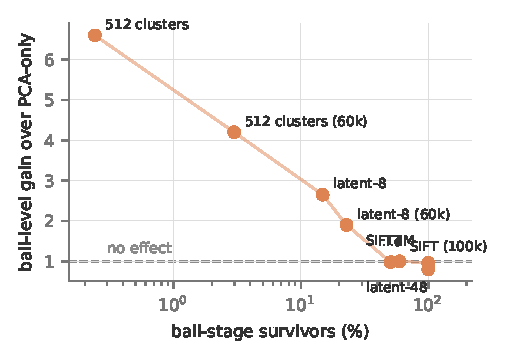
\includegraphics[width=0.92\linewidth]{fig_law.pdf}
\caption{The measured ball-value law across all eight datasets and trials
(parity code): the ball level's wall-clock gain over the PCA-only cascade
is a monotone function of its own pruning rate. The funnel's tier-3 trial
measures precisely the $x$-axis quantity, which is why it predicts
full-scale outcomes from a sample---including the negative verdicts below
the dashed line.}
\label{fig:law}
\end{figure}

\section{The Hybrid Algorithm}
\label{sec:algorithm}

\subsection{Offline}

Fit PCA (covariance accumulated in chunks, so no full
\texttt{float64} copy of the dataset is materialized), select the cascade
widths from the eigen curve (\S\ref{sec:funnel}), and fit $k$-means with
$k = \mathrm{clip}(\sqrt{N}, 64, 4096)$ (MiniBatch; 24\,s on SIFT1M for
$k{=}1024$). Store per point a cluster id (\texttt{int32}) and $d_p$
(\texttt{float32})---8 bytes---plus the $k \times d$ centroids and
per-cluster radii. A measured sweep over $k \in \{8, 64, 256, 1024, 4096\}$
on SIFT1M shows ball-stage survivors falling monotonically
(81\%$\to$43\%) while fit cost rises $4\,\mathrm{s} \to 47\,\mathrm{s}$;
$\sqrt{N}$ sits at the knee of the gain-versus-fit-cost curve, which is why
it is the default rather than a tuned constant.

\subsection{Query Pipeline}

\begin{enumerate}
\item $k$ centroid distances ($k \cdot d$ operations).
\item Ball bounds (\ref{eq:ball}) for all $N$ points: one gather and one
  absolute difference each.
\item \textbf{Probe}: exact distances to the \textsc{probe}$=50$ points with
  the smallest ball bounds seed a safe initial radius $r$ (the Top-50
  probe of \S\ref{sec:pca}, seeded by ball bounds instead of coarse
  projections).
\item Ball pruning: retain points with $\mathrm{bound}^2 < r^2$.
\item PCA cascade $(8,16,32,64)$ on the survivors, with a \textbf{re-probe}
  at the first PCA stage: before pruning, exact distances to the 50 best
  8-dimensional candidates tighten $r$. Without this step the ball-seeded
  radius is loose and the cascade degrades (8-D survivors 27.2\% versus
  14.6\% with it); with it, the cascade matches PCA-only tightness
  stage-for-stage.
\item Full-distance check on the final survivors. The result is provably
  identical to brute force, and is additionally verified against the
  official ground truth in every experiment.
\end{enumerate}

\subsection{Exact $k$-NN}
\label{sec:knn}

The pruning radius generalizes from the best evaluated distance to the
$k$-th smallest exact distance among points evaluated so far: the $k$-th
order statistic over a \emph{subset} can only overestimate the true one,
so any point whose lower bound reaches it provably cannot enter the
$k$-NN set. One subtlety carries an exactness bug if missed: the evaluated
multiset can contain a point twice (the probe and re-probe sets overlap),
and the $k$-th order statistic of a multiset with duplicates is biased
low---which \emph{over}-prunes. The minimum (the 1-NN special case) is
duplicate-invariant; the $k$-th order statistic is not, so the radius must
be taken over \emph{distinct} evaluated points. The probe size grows to
$\max(50, k)$ so the initial radius is a valid $k$-th statistic.
Correctness is verified against brute force across datasets, both cascade
paths, and $k$ up to $n-1$; a second subtlety surfaced in verification:
integer-valued descriptors make exact distance \emph{ties} real (SIFT
query~13 has two points at squared distance exactly 61334, only one of
which is in the official ground truth), so $k$-NN sets are unique only up
to ties at the boundary.

\subsection{Out-of-Core Layout}
\label{sec:layout}

Pruning fragments I/O only if the layout ignores it---the classic
index-versus-scan crossover: hundreds of scattered small reads can lose to
a full sequential scan. Our two-tier design keeps \emph{resident} only what
pruning decisions touch: the rotated sketch of the first
$\max(\mathrm{levels})$ PCA dimensions plus the ball metadata
(\texttt{assign}${+}d_p$, 8 bytes/point), centroids, and per-cluster
offsets---$2$--$8\times$ smaller than the data. Full-dimensional vectors
live on disk in two interchangeable files: original order (each fetch is
one small aligned read) and \emph{cluster-major} order, in which each
$k$-means cluster is a contiguous, page-aligned block ($<$0.4\% padding),
written sequentially into \texttt{fallocate}-preallocated extents. The
entire cascade---probe, re-probe, all pruning stages---runs on the resident
tier; the disk is touched only by the fetch set (probe $+$ re-probe $+$
finalists), whose exact membership \S\ref{sec:ooc} measures. Two structural
facts make the layout matter. First, the cluster-level bound alone is a
weak block-skipper (on SIFT1M, 40--52\% of clusters survive it). Second,
the fetch set is far more concentrated than uniform---nearest neighbors of
a query are near each other, so they share clusters---which converts the
final fetch into few large reads. This is the wisdom of the
VA-file~\cite{vafile}, SPANN~\cite{spann}, and DiskANN~\cite{diskann}:
sequential sketches, layout-aware fetches. The same $k$-means that supplies
the bound supplies the layout---and \S\ref{sec:ooc} shows it earns its keep
as a \emph{partitioner} even on datasets where the funnel rejects it as a
\emph{pruning level}.

\section{Evaluation}
\label{sec:eval}

\textbf{Metrics policy.} Primary claims are stated in hardware-independent
work units, because wall-clock proved regime-dependent: the same algorithm
measured $4.7\times$, $3.6\times$, $2.7\times$, and parity under changes of
numeric type, machine load, and implementation tuning, while its work counts
never moved (details below). The primary metrics are (1) full-vector fetches
per query (the out-of-core I/O currency), (2) total bytes touched per query,
\emph{charging the pruning machinery itself}, (3) resident RAM bytes per
vector, and (4) the survivor cascade, which is the algorithmic fingerprint.
Wall-clock appears as validation of a first-order cost model
($t \approx \mathrm{bytes}/\mathrm{bandwidth} +
\mathrm{ops}/\mathrm{throughput}$), with FAISS supplying the tuned-constants
reference---so a reader can plug their machine's constants into our work
numbers and predict their own outcome.

\textbf{Setup.} Intel i9-9900K (8C/16T, AVX2${+}$FMA, no AVX-512),
dual-channel DDR4, 30\,GB usable RAM; NVMe SSD measured under
\texttt{O\_DIRECT} at 2.04\,GiB/s sequential (8\,MiB reads) and 80\,\textmu s
per random 4\,KiB read; \texttt{faiss-cpu} 1.15 dispatching its AVX2 build;
NumPy and OpenBLAS at the AVX2 tier---baseline and FAISS use the same
instruction set. SIFT1M in-RAM timings (Table~\ref{tab:sift}) are medians
of 5 repetitions on a quiet machine with warm cache; the multi-dataset,
$k$-NN, and out-of-core tables are medians or means over 100 queries in a
single repetition on a quiet machine (work counts and byte counts are
exact and run-invariant; only the millisecond columns carry run noise).
Exactness is verified on every query of every experiment---against
official ground truth where one exists, against in-harness brute force
otherwise. Results are CPU-governor-insensitive (medians within 2\%).

\subsection{SIFT1M}

\begin{table}[t]
\caption{SIFT1M, 100 official queries, medians of 5 repetitions,
implementation parity. All methods return the ground-truth neighbor on
every query.}
\label{tab:sift}
\small
\begin{tabular}{@{}lrrl@{}}
\toprule
Method & ms/query & Speedup & Survivors per stage (\%) \\
\midrule
brute (NumPy) & 167.3 & 1.0$\times$ & --- \\
PCA-only & 61.1 & 2.7$\times$ & 14.7 / 5.2 / 0.8 / 0.06 \\
hybrid & 62.2 & 2.7$\times$ & ball 50.6 $\to$ 14.6 / 5.1 / 0.7 / 0.05 \\
\midrule
FAISS-flat, 1 thread & 29.3 & 5.7$\times$ & (scans 100\%) \\
FAISS-flat, batch-100 & 5.9 & 28$\times$ & (scans 100\%) \\
\bottomrule
\end{tabular}
\end{table}

\begin{figure}[t]
\centering
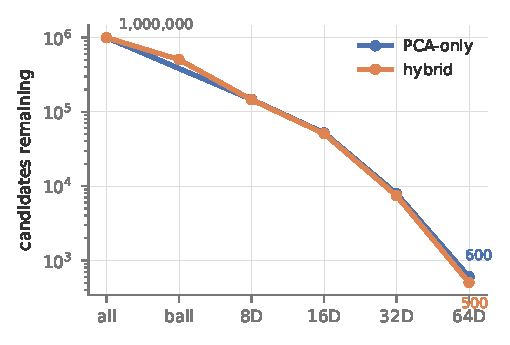
\includegraphics[width=0.92\linewidth]{fig_cascade.pdf}
\caption{Candidates remaining after each stage on SIFT1M (log scale,
average over 100 official queries). The cascade discards four orders of
magnitude before any full-distance evaluation; the hybrid enters the PCA
stages with half the population and finishes equally tight. This profile is
the algorithmic fingerprint: it was invariant under every change of numeric
type, machine load, and implementation tuning in this paper.}
\label{fig:cascade}
\end{figure}

Table~\ref{tab:sift} gives the in-RAM picture, and
Figure~\ref{fig:cascade} the cascade behind it. The PCA cascade alone reaches
$2.7\times$; \textbf{the ball level is a wall-clock tie on SIFT}---its
50\% pruning saves about what its bound computation costs---exactly as the
sample trial predicts (\textsc{skip}, \S\ref{sec:funnel}). The hybrid's
SIFT-side value is therefore out-of-core and residency only
(\S\ref{sec:layout}); the wall-clock case for the ball level rests on
clustered and low-intrinsic-dimension data (\S\ref{sec:regimes}). The
survivor cascade exactly reproduces the preliminary reports'.

\begin{table}[t]
\caption{Hardware-independent work per query on SIFT1M. Terms are
per-dimension $(x{-}y)^2$ evaluations; bound ops are per-point ball-bound
evaluations, charged separately. Counts derive analytically from the
survivor statistics (\texttt{count\_ops} in the repository)---an exhaustive
scan is $N \cdot d$ terms by definition, so no instrumentation of compiled
libraries is needed. These columns are identical on every machine and every
run.}
\label{tab:ops}
\small
\begin{tabular}{@{}lrrr@{}}
\toprule
Method & Terms (M) & Bound ops (M) & Terms vs brute \\
\midrule
brute / FAISS-flat & 128.0 & --- & 1.0$\times$ \\
PCA-only & 12.60 & 0 & \textbf{10.2$\times$} \\
hybrid & 8.67 & 1.00 & 14.8$\times$ \\
\bottomrule
\end{tabular}
\end{table}

Table~\ref{tab:ops} states the same experiment in the primary currency.
Three things the wall-clock hid become explicit. First, the cascade's
\emph{algorithmic} reduction is $10.2\times$---machine-free, and invariant
across every run in this paper, where the millisecond columns wobbled with
load. Second, FAISS-flat performs $10$--$15\times$ more work than the
cascade and still wins in-RAM wall-clock: the engineering-versus-algorithm
separation is now quantitative rather than rhetorical. Third, the hybrid
cuts terms further ($12.6 \to 8.7$\,M) but adds $1.0$\,M bound operations of
a different mix (gathers rather than streaming reads)---which is why its
wall-clock ties PCA-only despite the smaller term count, and why work
accounting that omits the pruning machinery would mislead.

FAISS \texttt{IndexFlatL2} wins the in-RAM race outright, scanning all
$10^6$ vectors in 29.3\,ms single-threaded. The gap is fusion, not SIMD:
both sides run AVX2, but FAISS's kernel makes one pass ($\sim$512\,MB of
traffic per query) where NumPy's expression materializes temporaries
($\sim$3 passes, 1.5--2\,GB), a $5.6\times$ advantage at identical work. The
comparison scopes the claim rather than defeating it: the cascade touches
$1{,}700\times$ fewer full vectors, requires 8--40 resident bytes per vector
against 512 for any flat scan, and its bounds compose with FAISS-grade
kernels rather than competing with them (the cascade could drive such a
kernel over its survivor sets). Disk-resident ANN systems occupy the same
economics but surrender exactness. Table~\ref{tab:resources} summarizes the
resulting three-way trade among speed, work, and the machine's most
expensive resource.

\begin{table}[t]
\caption{The exactness--speed--work--memory trade-off on SIFT1M (fp32,
$10^6 \times 128$). Flat scans must hold every vector resident
(512\,B/vector); the cascades keep only pruning metadata resident and page
full vectors from storage (\S\ref{sec:layout}): the 8-dimensional sketch
costs 32\,B/vector, the ball metadata 8\,B/vector. Parentheses give the
RAM saving relative to a flat scan. The last row situates disk-resident
ANN systems: their residency (taken from their own reports, not measured
here) is comparable to the cascades', but they answer the approximate
problem---the exact-at-cascade-residency quadrant is the one this work
occupies.}
\label{tab:resources}
\small
\begin{tabular}{@{}lcrrr@{}}
\toprule
Method & Exact & ms/query & Terms (M) & Resident RAM \\
\midrule
FAISS-flat, batch-100 & yes & 5.9 & 128.0 & 512\,MB \,(1$\times$) \\
FAISS-flat, 1 thread & yes & 29.3 & 128.0 & 512\,MB \,(1$\times$) \\
brute (NumPy) & yes & 167.3 & 128.0 & 512\,MB \,(1$\times$) \\
PCA-only & yes & 61.1 & 12.6 & 32\,MB \,(16$\times$) \\
hybrid & yes & 62.2 & 8.7\,{\small$+1.0$} & 8--40\,MB \,(13--64$\times$) \\
\midrule
IVF / disk ANN~\cite{faiss,diskann,spann} & no & --- & --- & $\sim$8--64\,MB \\
\bottomrule
\end{tabular}
\end{table}

\textbf{Why wall-clock is the wrong headline (measured).} Two confounds were
caught only by interrogating ratio changes. \emph{Numeric type}: sklearn's
PCA silently outputs \texttt{float64}, whose bandwidth-bound brute baseline
is $1.86\times$ costlier; a $2\times2$ decomposition on identical code
measures the same cascade at $3.6\times$ (f64---the first preliminary
report's regime, matching
its reported $4.3\times$) versus $2.7\times$ (f32). \emph{Implementation
parity}: an unnecessary full-array gather in our own PCA-only path inflated
the ball level's apparent contribution to $2.0\times$; fixing it revealed
the tie in Table~\ref{tab:sift}. Machine load adds a further multiplier:
background bandwidth contention slows the scan-bound baseline most,
flattering all pruners. Survivor counts were invariant through every one of
these changes. Hence the metrics policy.

\subsection{Four Real Datasets: the Gain Grows with Dimension}
\label{sec:datasets}

\begin{table}[t]
\caption{Exact 1-NN at full scale, eigen-curve-selected levels, PCA-only
cascade. Terms count per-dimension $(x{-}y)^2$ evaluations; a scan is
$n \cdot d$ by definition. All queries exact.}
\label{tab:datasets}
\small
\begin{tabular}{@{}lrrrrr@{}}
\toprule
Dataset & $n$ & $d$ & Wall & Terms (M) & Work red. \\
\midrule
SIFT1M & $10^6$ & 128 & 2.6$\times$ & 12.6 & 10.2$\times$ \\
GIST1M & $10^6$ & 960 & \textbf{6.2$\times$} & 46.1 & \textbf{20.8$\times$} \\
DBpedia-OpenAI & $10^6$ & 1536 & 6.0$\times$ & 119.6 & 12.8$\times$ \\
DEEP10M & $10^7$ & 96 & 1.2$\times$ & 244.0 & 3.9$\times$ \\
\bottomrule
\end{tabular}
\end{table}

Table~\ref{tab:datasets} answers the question SIFT alone cannot: does
anything beyond SIFT prune? Everything measured does, and the wall-clock
gain \emph{grows} with dimensionality---$2.6\times$ at 128-D,
$6.2\times$ at 960-D, $6.0\times$ at 1536-D---because brute force pays the
full dimension for every point while the cascade pays for intrinsic
structure. The result that mattered most in prospect: modern learned
embeddings (DBpedia abstracts under OpenAI \texttt{ada-002}), whose flat
spectra (664 of 1536 dimensions for 95\% variance) looked like the
approach's natural failure mode, prune to 0.64\% finalists once the
cascade widths respect the eigen curve (\S\ref{sec:funnel})---with the
\emph{fixed} $(8,16,32,64)$ ladder the same data measures $1.3\times$ and
reads as unprunable. DEEP10M is the honest boundary case: 96 dimensions of
already-PCA-compressed deep features leave a $3.9\times$ work reduction
but only $1.2\times$ in-RAM wall-clock; the funnel's sample verdict
(\textsc{moderate}, ``useful out-of-core'') says exactly this in advance,
and \S\ref{sec:ooc} confirms where its value lives. On all four datasets
the ball level's sample verdict (\textsc{skip} everywhere; survivor rates
50--99\%) was confirmed at full scale---the ball-value law of
\S\ref{sec:funnel} holding on real data at $10^6$--$10^7$ points.

\subsection{Exact $k$-NN}
\label{sec:knn-eval}

\begin{table}[t]
\caption{Exact $k$-NN, PCA-only cascade, wall-clock speedup over brute
force and (in parentheses) work reduction in terms. All queries exact;
$k{=}100$ additionally matches official ground truth up to boundary ties.}
\label{tab:knn}
\small
\begin{tabular}{@{}lrrr@{}}
\toprule
Dataset & $k=1$ & $k=10$ & $k=100$ \\
\midrule
SIFT1M & 2.6$\times$ (10.2$\times$) & 1.9$\times$ (6.2$\times$) & 0.7$\times$ (1.6$\times$) \\
GIST1M & 6.2$\times$ (20.8$\times$) & 4.0$\times$ (10.3$\times$) & 0.9$\times$ (1.5$\times$) \\
DBpedia-OpenAI & 6.0$\times$ (12.8$\times$) & 3.1$\times$ (5.8$\times$) & 0.8$\times$ (1.2$\times$) \\
DEEP10M & 1.2$\times$ (3.9$\times$) & 0.8$\times$ (2.0$\times$) & 0.3$\times$ (0.6$\times$) \\
\bottomrule
\end{tabular}
\end{table}

Table~\ref{tab:knn} reports the $k$-NN generalization
(\S\ref{sec:knn}) with deliberate honesty: the method wins to
$k \approx 10$ and \emph{loses} in-RAM wall-clock at $k = 100$ on every
dataset. The mechanism is structural, not incidental: the pruning radius
is the $k$-th best distance, which grows with $k$, and survivor counts
grow with it---at $k{=}100$ the ball stage passes 99--100\% and the
cascade approaches a scan with overhead. The $k{=}100$ work reductions
($1.2$--$1.6\times$ on the million-scale sets) still translate to fewer
bytes fetched out of core, which is where large-$k$ exact queries should
run (\S\ref{sec:ooc}).

\subsection{Structure Regimes}
\label{sec:regimes}

\begin{table}[t]
\caption{Structure regimes (synthetic, $n=200$k, $d=64$ for the first two;
$n=60$k, $d=128$ for the funnel rows), implementation parity. ``Ball
survivors'' is the ball stage's own pruning rate---the quantity the funnel's
trial measures.}
\label{tab:regimes}
\small
\begin{tabular}{@{}lrrrl@{}}
\toprule
Dataset & PCA-only & Hybrid & Ball surv. & Verdict \\
\midrule
512 tight clusters & 2.1$\times$ & \textbf{13.9$\times$} & 3\% & \textsc{add} \\
latent-8 Gaussian & 2.1$\times$ & 5.6$\times$ & 15--23\% & \textsc{add} \\
SIFT1M & 2.7$\times$ & 2.7$\times$ & 50--59\% & \textsc{skip} \\
latent-48 Gaussian & 1.9$\times$ & 0.8$\times$ of PCA & 100\% & \textsc{skip} \\
i.i.d.\ Gaussian & 0.3$\times$ & --- & 100\% & \textsc{skip} (all) \\
\bottomrule
\end{tabular}
\end{table}

Table~\ref{tab:regimes} spans the design space, negative results included
deliberately. On the flat-spectrum clustered dataset---PCA's blind
spot---the ball level prunes to 3\% before any projection is computed and
the hybrid reaches $13.9\times$; its bound requires no multiplications, so
it undercuts even the 8-dimensional scan. On the latent-48 blob the ball
level is measured to \emph{hurt} ($0.8\times$: 100\% survivors, pure
overhead), and on i.i.d.\ noise the diagnostic correctly reports that
nothing works and brute force or ANN should be used. The i.i.d.\ row also
shows the PCA cascade itself losing to brute force ($0.3\times$)---the
honest boundary of the entire approach.

\subsection{Extrapolation}
\label{sec:extrap}

The funnel's trial on a 100k SIFT sample returns $1.0\times$
(\textsc{skip}); the full-1M parity benchmark measures exactly that (61.1
versus 62.2\,ms). The check extends to every dataset: GIST1M
sampled at $9.3\times$ work with the fixed ladder and $15.2\times$ with
eigen-curve levels; the full-1M runs measured $13.1\times$ and
$20.8\times$ respectively (the sample is conservative). DEEP10M sampled
\textsc{moderate} at $3.6\times$
and measured $3.9\times$ at $10^7$ points; the ball level's sample
\textsc{skip} was confirmed at full scale on all four datasets
(e.g.\ GIST: 92\% ball survivors, identical term counts, strictly worse
wall-clock). The diagnostic predicts full-scale outcomes from a
sample---including the negative verdicts, which is its most valuable
behavior: it prevents building a useless level.

\subsection{Out of Core: Measured Cold Reads}
\label{sec:ooc}

\begin{table}[t]
\caption{Cold-read exact 1-NN under \texttt{O\_DIRECT} (every byte from
the device; page cache bypassed, so each query is cold by construction).
Scan streams the whole file; point fetches each needed vector from the
original-order file; block fetches whole clusters from the cluster-major
file. All arms return identical exact results.}
\label{tab:ooc}
\small
\begin{tabular}{@{}llrrr@{}}
\toprule
Dataset & Arm & ms/query & MB/query & Reads \\
\midrule
SIFT1M       & scan  & 402  & 488  & 62 \\
(488\,MB)    & point & \textbf{61} \,(7$\times$) & \textbf{2.3} \,(212$\times$) & 588 \\
             & block & 81 \,(5$\times$) & 37 & 73 \\
\midrule
GIST1M       & scan  & 3006 & 3663 & 458 \\
(3.6\,GiB)   & point & \textbf{421} \,(7$\times$) & \textbf{91} \,(40$\times$) & 12{,}379 \\
             & block & 751 \,(4$\times$) & 1224 & 158 \\
\midrule
DBpedia      & scan  & 5385 & 5860 & 733 \\
(5.7\,GiB)   & point & \textbf{318} \,(\textbf{17$\times$}) & \textbf{8.0} \,(\textbf{730$\times$}) & 1028 \\
             & block & 418 \,(13$\times$) & 374 & 36 \\
\midrule
DEEP10M      & scan  & 3574 & 3664 & 458 \\
(3.6\,GiB)   & point & 1542 \,(2$\times$) & \textbf{209} \,(18$\times$) & 50{,}356 \\
             & block & \textbf{1378} \,(3$\times$) & 780 & 223 \\
\bottomrule
\end{tabular}
\end{table}

Section~\ref{sec:layout} motivated the two-tier layout from structure;
Table~\ref{tab:ooc} measures it end to end. The protocol: all reads use \texttt{O\_DIRECT}
with page-aligned buffers, so the page cache is bypassed and every query
pays device prices---a cold-cache protocol with no cache-flushing
ceremony, deliberately conservative on NVMe, where cheap random reads and
high sequential bandwidth both favor the \emph{scan} baseline.

Three findings. \textbf{First, the headline}: on the OpenAI embeddings,
exact cold-read 1-NN takes 318\,ms against a 5.4-second scan
($17\times$), reading 8\,MB instead of 5.9\,GB ($730\times$ fewer bytes).
The byte ratios are device-independent; on storage slower or more
seek-bound than NVMe they translate to larger time ratios.
\textbf{Second, the fetch set is highly cluster-local}: the embeddings'
$\sim$1{,}014 fetched points occupy a median of 27 of 1024 clusters
(uniform placement would touch $\sim$644); SIFT's 583 points occupy 52.
Nearest neighbors of a query are near each other. This is what makes the
cluster-major arm viable at all---and it means the $k$-means structure
earns residence as a \emph{partitioner} even where the funnel rejects its
\emph{bound} (\textsc{skip} on all four datasets): the same geometry,
useless for compute, valuable for layout. \textbf{Third, point-versus-block
is a device property}: with serial reads at 80\,\textmu s the point arm's
few thousand small fetches beat the block arm's fewer-but-heavier reads on
three of four datasets, and only DEEP10M's 50k-point fetch set flips the
order. Parallel small reads (NVMe queue depths reward exactly this) would
extend the point arm's advantage; seek-bound media would flip every row
toward block. The layout writes both files; the diagnostic should pick per
device.

One design lesson surfaced only here: \emph{the optimal cascade depth is
deeper out of core than in RAM}. SIFT's eigen-curve levels $(8,16,40)$
minimize in-RAM terms but fetch 3{,}381 points; the deeper $(8,16,32,64)$
ladder spends more sketch terms to fetch only 588---and wins the cold-read
benchmark ($61$ vs $91$\,ms). In-RAM, terms are the currency; out of core,
fetched bytes are, and the level-selection objective should follow the
medium.

\subsection{Baseline: ADSampling}
\label{sec:ads}

\begin{table}[t]
\caption{ADSampling (faithful NumPy port of the reference implementation,
$\epsilon_0{=}2.1$, $\Delta d{=}32$) versus our PCA-only cascade, $k=1$.
Work in millions of dimension-terms per query; recall under
float64-verified ground truth. Ours is exact by construction.}
\label{tab:ads}
\small
\begin{tabular}{@{}lrrr@{}}
\toprule
Dataset & ADS terms (recall) & Ours (exact) & Winner \\
\midrule
SIFT1M & 33.0 \,(1.000) & \textbf{12.6} & ours 2.6$\times$ \\
GIST1M & \textbf{44.5} \,(1.000) & 46.1 & tie \\
DBpedia-OpenAI & \textbf{49.8} \,(1.000) & 119.6 & ADS 2.4$\times$ \\
DEEP10M & 325.8 \,(1.000) & \textbf{244.0} & ours 1.3$\times$ \\
\bottomrule
\end{tabular}
\end{table}

ADSampling~\cite{adsampling} is the natural adversary: it also prunes with
incremental prefix distances after a rotation, but its rotation is random
(partial distances become unbiased samples) and its stopping rule is a
sequential hypothesis test with tunable error rate $\epsilon_0$---harder
pruning per dimension, bought with the exactness guarantee. We ported the
reference implementation to the same harness and currency (dimensions
touched $=$ terms) for parity. Table~\ref{tab:ads} is honestly mixed
in-RAM: we win at 96--128 dimensions, ADS wins on the 1536-D embeddings,
GIST ties; at $k{=}10$ ADS widens its advantage. On recall we correct our
own first measurement: an earlier float32 ground-truth check miscounted
near-duplicate points (catastrophic cancellation) as recall failures;
under float64 verification ADS at default $\epsilon_0$ achieved perfect
recall on every $k{=}1$ query we ran, with one true neighbor missed in
600 query-tasks (GIST, $k{=}10$, recall 0.9990). The distinction that
matters is therefore \emph{guarantee versus empirical}, not observed
failure---and it is structural, since no $\epsilon_0$ makes the test a
bound.

The decisive difference is not in RAM. ADS pays its $\Delta d = 32$
floor for \emph{every} point in the dataset---SIFT's 33.0M and DEEP10M's
325.8M terms sit exactly at $32n$---so it must touch every vector, and
out of core it reads full-scan bytes regardless of parameters (its
successor PDX~\cite{pdx} restructures the layout dimension-major but
still visits every vector). Our cascade fetches 0.06--1\% of vectors
(Table~\ref{tab:ooc}). The methods also compose rather than compete: a
statistical test could accelerate the final full-distance checks over our
survivor sets, at the usual price.

\section{Limitations}

High \emph{intrinsic} dimensionality defeats every cheap bound: distance
concentration flattens the eigenvalue spectrum and the spread of $d_p$
simultaneously, and the funnel exists precisely to detect this and say so
(Table~\ref{tab:regimes}, last row); DEEP10M sits near this boundary in
RAM. In-RAM wall-clock at native-code constants belongs to fused
exhaustive scans (FAISS) at the 128-D scale, and ADSampling's statistical
pruning beats our deterministic bounds in-RAM on the highest-dimensional
embeddings (\S\ref{sec:ads}). Exact $k$-NN loses in-RAM wall-clock by
$k = 100$ on every dataset we measured (\S\ref{sec:knn-eval}). The
out-of-core measurements use \texttt{O\_DIRECT} on datasets that fit in
RAM---valid device-price accounting, but a
larger-than-RAM run (with parallel rather than serial fetch I/O) remains
future work, as do updates: the cluster-major layout assumes a static,
rebuild-periodically index, the same assumption disk-ANN builds make.
Ball-bound and layout quality depend on the $k$-means sample as any
learned structure does, though correctness never does.

\section{Conclusion}

Exact lower bounds are shapes; shapes compose; and the right composition is
a property of the data, measurable on a sample before any index is built.
On that principle this paper delivers an exact $k$-NN index that configures
itself end to end---cascade widths from the eigenvalue curve (without which
1536-dimensional embeddings masquerade as unprunable), levels from a
measured trial whose sample verdicts are confirmed at $10^6$--$10^7$ scale
on four real datasets, honest breaking points stated ($k = 100$ in RAM;
i.i.d.\ data everywhere)---and an out-of-core argument that has become a
measurement: exact cold-read queries $7$--$17\times$ faster than a disk
scan at $40$--$730\times$ fewer bytes, against a state-of-the-art
statistical pruner that structurally cannot leave RAM. The recurring lesson
of this work is that every constant we had silently tuned to one
dataset---cascade widths, verdict thresholds, even our own ground-truth
checker---failed on the next one, and every fix was the same: derive it
from a measurement. Measure the data to choose the index; count the work to
predict the time.

\vspace{1ex}
\noindent\textbf{Artifact.} Code, diagnostics, and all experiment scripts:\\
\texttt{github.com/taiwuchiang-gmail/hierarchical-pca-search}

\bibliographystyle{ACM-Reference-Format}
\bibliography{references}

\end{document}
